% This is auto-generated file: do not edit!
% Exported from microMathematics Plus, version 2.15.6


Agora desenharemos várias funções dadas
no sistema de coordenadas polares.
Cada ponto neste sistema é determinado
por uma distância r da origem e o
ângulo f do eixo x.
\begin{center}\begin{tabular}{c} 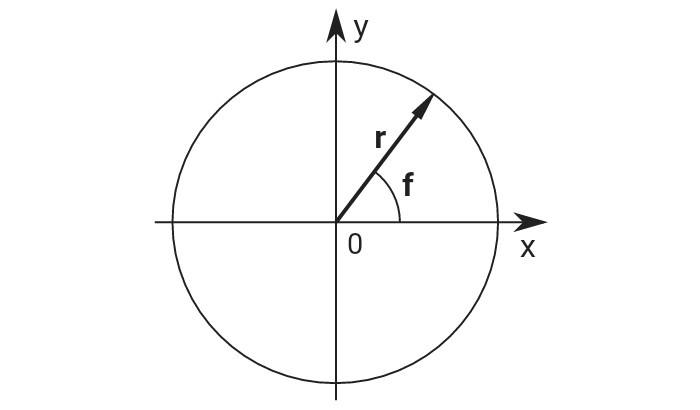
\includegraphics[resolution=320]{graphics/polar_plot_fig1.png} \end{tabular}\end{center}

O ângulo f é nossa variável
independente que muda como está a
seguir:
\begin{center}\begin{tabular}{c}
  $f := \left[ 0.01,\, 0.05 \,..\, 300 \right]$
\end{tabular}\end{center}

A distância r(f) é a nossa variável
dependente. Tendo um par de f e r, nós
podemos tranformar em coordenadas
Cartesianas x e y usando as funções
seno e cosseno:
\begin{center}\begin{tabular}{cc}
  $x(r) := r \cdot cos \left( f\right) $ &
  $y(r) := r \cdot sin \left( f\right) $ \cr
\end{tabular}\end{center}

\subsection{Um caracol}

Definiremos nossa funcção polar em três
passos. A primeira expressão define
uma ''roda'':
\begin{center}\begin{tabular}{ccc}
  $A := 1.1$ &
  $B := 1.271$ &
  $q := 2$ \cr
\end{tabular}\end{center}
\begin{center}\begin{tabular}{c}
  $r1(f) := A + 2 \cdot {sin \left( B \cdot f\right) }^{q}$
\end{tabular}\end{center}

Para desenhar esta função, adicionamos
e caixa de desenho usando o boão ''Novo
elemento'' na barra de ações ou o botão
''Adicionar desenho de função'' a partir
da barra de ferramentas:
\begin{center}\begin{tabular}{c} 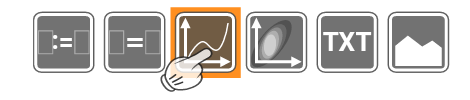
\includegraphics[resolution=320]{graphics/polar_plot_fig2.png} \end{tabular}\end{center}

Ao invés de f e r, usamos aqui regras
previamente definidas para
transformação x e y, onde r1(f) é
usado como um argumento simbólicopara
estas regras:
\begin{center}\begin{tabular}{c} 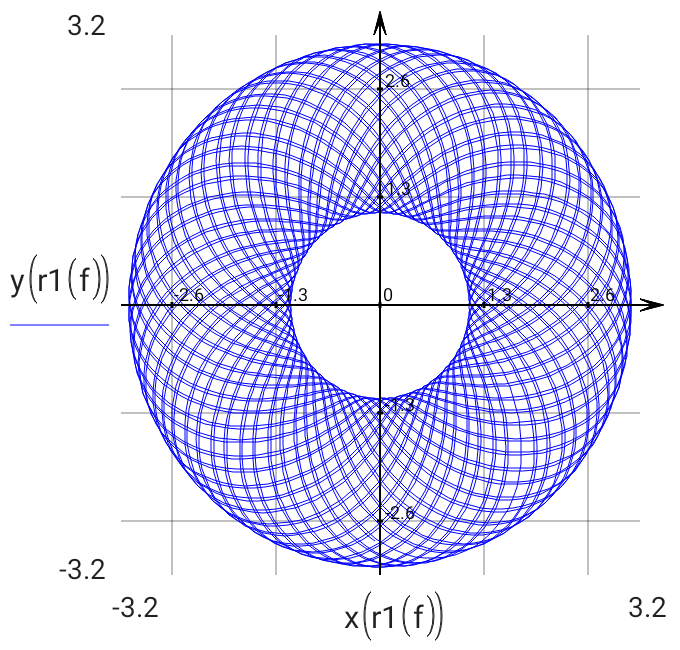
\includegraphics[resolution=320]{graphics/polar_plot_fig3.png} \end{tabular}\end{center}

Então, podemos alterar esta roda como
segue:
\begin{center}\begin{tabular}{c}
  $r2(f) := A + 2 \cdot {sin \left( B \cdot f + 1 \cdot r1 \left( f\right) \right) }^{q}$
\end{tabular}\end{center}
\begin{center}\begin{tabular}{c} 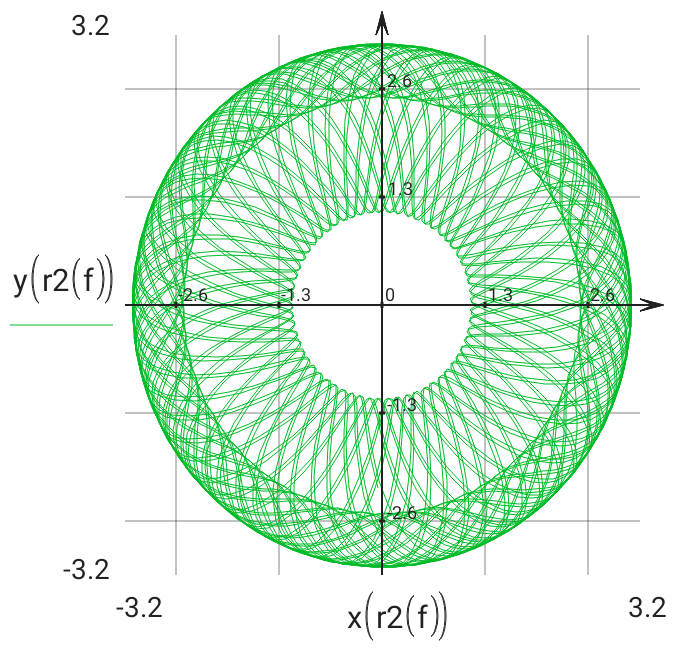
\includegraphics[resolution=320]{graphics/polar_plot_fig4.png} \end{tabular}\end{center}

Finalmente, fazemos a escala da última
função r2(f) usando uma conversão de
inteiro para flutuante que parece uma
função em escada. Como resultado,
obtemos um belo caracol:
\begin{center}\begin{tabular}{c}
  $r(f) := r2 \left( f\right)  \cdot floor \left( f\right)  / 10$
\end{tabular}\end{center}
\begin{center}\begin{tabular}{c} 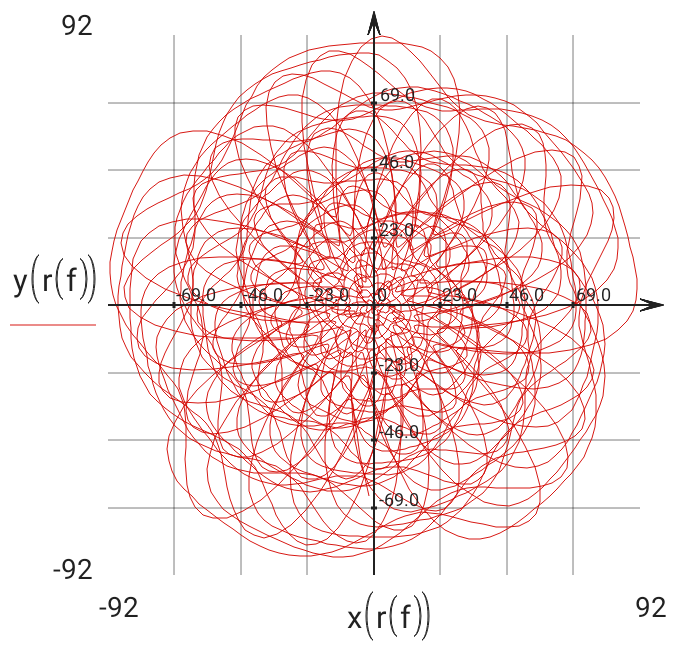
\includegraphics[resolution=320]{graphics/polar_plot_fig5.png} \end{tabular}\end{center}

\subsection{Japanese Maple}

O Maple japonês é muito conhecido pela
forma e cores atraentes de suas
folhas. Estas folhas podem ser
descritas matematicamente e desenhadas
como uma curva no sistema de
coordenadas polares:
\begin{center}\begin{tabular}{c}
  $f := \left[ 0.01,\, 0.02 \,..\, 100 \right]$
\end{tabular}\end{center}
\begin{center}\begin{tabular}{cc}
  $x(r) := r \cdot cos \left( f\right) $ &
  $y(r) := r \cdot sin \left( f\right) $ \cr
\end{tabular}\end{center}
\begin{center}\begin{tabular}{c}
  $s1(f) := \left( 1 + sin \left( f\right)  \right) \cdot \left( 1 - 0.9 \cdot  \left| sin \left( 4 \cdot f\right)  \right|  \right)$
\end{tabular}\end{center}
\begin{center}\begin{tabular}{c}
  $s2(f) := 0.9 + 0.05 \cdot cos \left( 200 \cdot f\right) $
\end{tabular}\end{center}
\begin{center}\begin{tabular}{c}
  $r(f) := floor \left( f\right)  \cdot s1 \left( f\right)  \cdot s2 \left( f\right)  + rnd \left( 2\right)  - 1$
\end{tabular}\end{center}
\begin{center}\begin{tabular}{c} 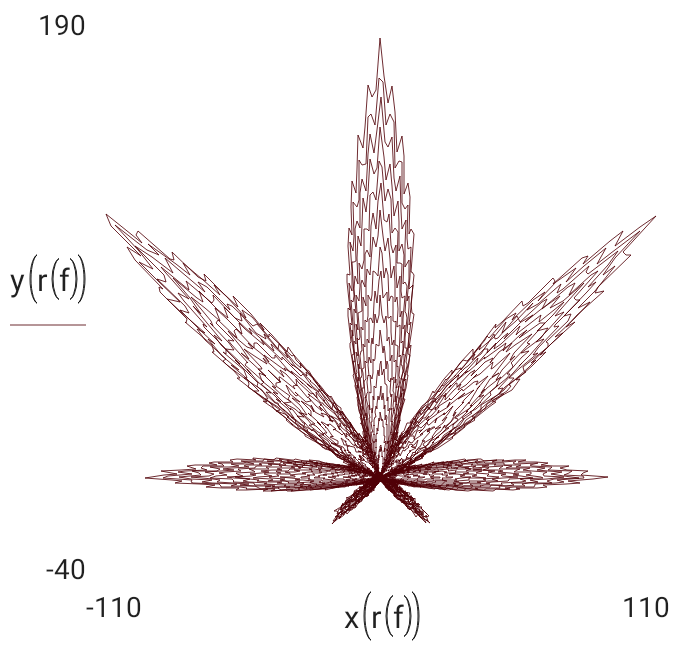
\includegraphics[resolution=320]{graphics/polar_plot_fig6.png} \end{tabular}\end{center}

http://en.wikipedia.org/wiki/Acer\_palmatum